%!TEX output_directory = texaux
%!TEX spellcheck
%!TEX root = ../main.tex

\setlength{\abovedisplayskip}{20pt}
\setlength{\belowdisplayskip}{20pt}

\chapter{Generowanie dialogu}\label{rozdzial3}

Dialog opisujemy jako ciąg $U_1, U_2, \dots, U_K$ wypowiedzi w języku naturalnym. Każda wypowiedź jest sekwencją słów. Tak jak poprzednio korzystamy ze znaczników $\mathbf{start}$ i $\mathbf{end}$. Naginając nieco zapis:
\[U_k = {w_k}_1^{T_k} = (\mathbf{start}={w_k}_1, {w_k}_2, {w_k}_3, \dots, {w_k}_{T_k}=\mathbf{end})\]

\noindent
Rozszerzając przypadek pojedynczych sekwencji, możemy napisać
\[
\begin{aligned}
\hat{P}(U_1^K) &= \prod\limits_{k=1}^K \hat{P}(U_k \mid U_1^{k-1}\, ;\, \theta)\\
               &= \prod\limits_{k=1}^K \prod\limits_{t=1}^{T_k}
                  \hat{P}({w_k}_t \mid {w_k}_1^{t-1}, U_1^{k-1}\, ;\, \theta)
\end{aligned}
\]

Możemy wykorzystać \textit{RNNLM} do modelowania dialogu konkatenując poszczególne wypowiedzi. Otrzymany ciąg $U_1^\frown U_2^\frown \cdots^\frown U_K$ traktujemy jak jedną sekwencję. Niekoniecznie jest to jednak najlepsza metoda. W dalszej części rozdziału przedstawię opisany w \cite{serbanhred} model, który radzi sobie trochę lepiej. Pokażę też, jak wyglądały dialogi generowane przez moją implementację.

%%%%%%%%%%%%%%%%%%%%%%%%%%%%%%%%%%%%%%%%%%%%%%%%%%%%%%%%%%%%%%%%%%%%%%%%%

\section{Dostępność danych}

Zanim przystąpimy do optymalizacji modeli, trzeba zdobyć materiał uczący. Znalezienie dużej liczby publicznie dostępnych tekstów, szczególnie w języku angielskim, nie stanowi ogromnego problemu, nawet dla pojedynczych osób. Wszystkie artykuły Wikipedii są regularnie udostępniane w wygodnym formacie w postaci możliwych do pobrania zrzutów. Common Crawl\footnote{\url{http://commoncrawl.org/}} daje możliwość analizy zawartości blisko 3 miliardów stron internetowych. Dzieła literackie, archiwa gazet, cyfrowe zbiory bibliotek, ze wszystkich tych źródeł można korzystać za darmo.

Jeśli chcemy jednak znaleźć dane dialogowe mogące posłużyć do trenowania chatbota, sprawy mają się nieco inaczej. Duże zbiory danych istnieją, ale tym, z~którymi się spotkałem, sporo brakuje do statusu idealnego źródła.

\begin{itemize}
    \item \textbf{MovieTriples} \cite{serbanhred}\\[3pt]
    Zbiór napisów filmowych. W jego skład wchodzi 250\,000 trójek wypowiedzi. Każda trójka stanowi spójny fragment większego dialogu. Dane są udostępniane przez autorów na życzenie.

    \item \textbf{SubTle} \cite{subtle}\\[3pt]
    Kolejny, większy zbiór napisów do filmów. Gromadzi skrypty 5\,764 filmów, co przekłada się na 5,5 miliona pełnych tur dialogowych, czyli par kolejnych wypowiedzi. Podobnie jak \textit{MovieTriples}, dostępny na życzenie.

    \item \textbf{Ubuntu Dialogue Corpus} \cite{ubuntu}\\[3pt]
    Około 1 miliona dialogów dotyczących problemów technicznych nękających użytkowników Ubuntu. Korpus jest publicznie dostępny\footnote{\url{https://irclogs.ubuntu.com/}}.

    \item \textbf{\st{Twitter}} \cite{snapdata}\\[3pt]
    Do niedawna Uniwersytet Stanforda udostępniał kolekcję tweetów z drugiej połowy 2009 roku. Liczyła ona 467 milionów wiadomości. Niestety na prośbę Twittera zbiór musiał zostać usunięty z Internetu.

    \item \textbf{Reddit}\\[3pt]
    Istnieje możliwość pobrania liczącego setki gigabajtów zrzutu\footnote{\url{https://bigquery.cloud.google.com/dataset/fh-bigquery:reddit_comments}} komentarzy z~forum Reddit\footnote{\url{https://www.reddit.com/}}.
\end{itemize}

Problemem tych zbiorów danych jest bardzo silne zanurzenie w kontekście. Fakt ten czyni zadanie przewidywania odpowiedzi bardzo trudnym, nawet dla człowieka. Podejmujemy się zadania modelowania dialogu na podstawie samego tekstu, podczas gdy wypowiedzi uczestników rozmowy są podyktowane także innymi czynnikami. W przypadku filmów na zrozumienie przekazu składają się nie tylko wymiany zdań bohaterów, lecz także ton ich głosu, gestykulacja, sytuacja, w której się znajdują, czy wreszcie cała reszta filmu, którą widz zna, a o której sieć neuronowa nie ma pojęcia.

\textit{Ubuntu Dialogue Corpus} ma tę zaletę, że zapisy rozmów zawierają wszystkie niezbędne informacje. Użytkownicy komunikują się tylko za pomocą tekstu, a problem, z~którym się zmagają, jest opisany w rozmowie. To daje osobie zaznajomionej z~tematem możliwość pełnego zrozumienia dialogu. Wadą tych danych natomiast jest ich tematyka. Rozwiązywanie problemów technicznych wymaga dogłębnej wiedzy i~umiejętności wnioskowania, której maszyna czytająca forum się nie nauczy. O ile, choć z trudem, można wyobrazić sobie robota powtarzającego zapamiętane odpowiedzi na najczęściej pojawiające się pytania, o tyle przydatność chatbota w~analizie jakiegokolwiek niestandardowego zjawiska byłaby znikoma. Z drugiej strony dane zawierają wyłącznie rozmowy techniczne, więc robot będzie korzystał z dość hermetycznego języka informatycznego. Jeśli zadamy sobie pytanie: o czym taki program miałby rozmawiać?, to wszystko wydaje się prowadzić do sprzecznych celów.

Tweety również nie są zawieszone w próżni. Zwykle stanowią komentarz do wydarzenia znanego przynajmniej jednej ze stron, często mają charakter informacyjny. Czasami łączą się w krótkie rozmowy, co połączone z limitem 140 znaków daje pewne nadzieje, ale niestety nie miałem okazji tego sprawdzić.

Reddit nie posiada ograniczenia długości wiadomości. Powoduje to konieczność odfiltrowania rozmów, w których pojawiają się długie wypowiedzi; w przypadku czatu nie miałyby one racji bytu. Poza tym każdy wątek na Reddicie jest osadzony w kontekście, który stanowi pierwszy post. Raczej rzadko bywa to po prostu krótkie pytanie ogólne. Kontekst może być dość konkretnym tekstem, linkiem, często nawet obrazkiem lub filmem, co sprawia, że przewidywanie odpowiedzi bez niego staje się wręcz niemożliwe.

Swoje implementacje uczyłem na \textit{MovieTriples} i \textit{SubTle}. Z jednej strony dlatego, że były one wykorzystane w \cite{serbanhred}, więc wynik na nich stanowiłby dla mnie weryfikację poprawności kodu. Z drugiej strony są one względnie małe, więc proces uczenia modeli był na tyle krótki, że mogłem go wielokrotnie powtarzać.

%%%%%%%%%%%%%%%%%%%%%%%%%%%%%%%%%%%%%%%%%%%%%%%%%%%%%%%%%%%%%%%%%%%%%%%%%

\section{Model hierarchiczny}
Ta sekcja stanowi opis wykorzystanej w \cite{serbanhred} hierarchicznej architektury rekurencyjnej (ang. \textit{Hierarchical Recurrent Encoder-Decoder, HRED}) \cite{hred} do modelowania dialogu.

Oryginalnie \textit{HRED} miał służyć do przewidywania haseł, które użytkownik może wpisać w wyszukiwarce. Mechanizm zgadujący zapytania miał brać pod uwagę historię wyszukiwania, która mogła być dowolnie długa. Autorzy proponują podejście dwuetapowe: potraktować każde zapytanie jako osobną sekwencję, a całą historię jako ciąg zapytań. Ułatwi to sieci znajdowanie zależności pomiędzy całymi hasłami poprzez zredukowanie liczby kroków obliczeń mających miejsce między początkami dwóch kolejnych ciągów.

%%%%%%%%%%%%%%%%%%%

\subsection{Architektura \textit{encoder-decoder}}
W poprzednim rozdziale tekst generowany za pomocą \textit{RNNLM} miał przypominać tekst wejściowy. Generator był nie tylko deterministyczny, ale również w żaden sposób nie uwarunkowany. Wynik zależał wyłącznie od $\theta$ i od początkowego stanu sieci rekurencyjnej, $h_0$. Niektóre zastosowania wymagają generowania sekwencji zupełnie odmiennych od tekstu wejściowego, ale w pewien sposób z nim powiązanych. Za przykład niech posłuży tłumaczenie maszynowe, gdzie na podstawie zdania w~jednym języku chcemy, zachowując znaczenie, wyprodukować zdanie w drugim. Załóżmy, że chcemy uzależnić model od pewnego warunku początkowego $A$:
\[P(w_1^T) = \prod\limits_{t=1}^T P(w_t \mid w_1^{t-1}, A)\]

Odpowiednia modyfikacja \textit{RNNLM} pozwala osiągnąć ten cel. Zachowaniem generatora można sterować poprzez zmianę $h_0$. Wystarczy, że będziemy potrafili zakodować $A$ jako pewne $a \in \mathbb{R}^m$, gdzie $m$ jest wymiarem stanu sieci rekurencyjnej. Wówczas pozostaje tylko ustawić $h_0 := a$.

W przypadku pracy z tekstem, warunkiem początkowym będzie oczywiście jakaś sekwencja słów $A = a_1^{T_a}$. Żeby ją zakodować w $\mathbb{R}^m$ możemy wykorzystać drugą sieć rekurencyjną. Oznaczmy jej kolejne stany przez $s_1^{T_a}$. Można myśleć, że $s_i$ jest podsumowaniem sekwencji $a_1^i$. Ponieważ reprezentacją $A$ ma być pojedynczy wektor, będzie nas interesował wyłącznie ostatni stan. Ciąg $A$ kodujemy jako $s_{T_a}$.

Mamy więc dwa ciągi wejściowe: źródłowy $a_1^{T_a}$ i docelowy $w_1^T$. Zmodyfikowana architektura wygląda tak:
\begin{enumerate}
    \item \textbf{Warstwa zanurzeń}: identyczna jak w \textit{RNNLM}, ale zanurzamy obie sekwencje. Warstwa przerabia $a_1^{T_a}$ na ciąg wektorów $x_1^{T_a}$ oraz $w_1^T$ na $y_1^T$.
    \item \textbf{Kodujący \textit{RNN}}: przechodzi po $x_1^{T_a}$ i oblicza $s_{T_a}$.
    \item \textbf{Dekodujący \textit{RNN}}: czyta $y_1^T$ i produkuje ciąg stanów $h_1^T$, startując ze stanu początkowego $h_0 = s_{T_a}$.
    \item \textbf{Softmax}: tak jak w \textit{RNNLM}, $h_0^{T-1}$ jest przekształcane na ciąg $p_1^T$ rozkładów prawdopodobieństwa na $V$, tym razem zależnych od $A$.
\end{enumerate}

\begin{figure}[ht]
  \centering
    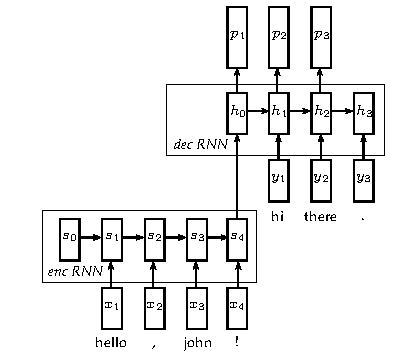
\includegraphics[width=0.8\textwidth]{chapter3/img/encdec.eps}
  \caption{\small{Przetwarzanie pary dialogowej przez \textit{encoder-decoder}. Dla czytelności warstwa zanurzeń została pominięta.}}
\end{figure}

Podobnie jak w \textit{RNNLM}, optymalizujemy parametry minimalizując \textit{nll} na ciągu docelowym, czyli
\[-\sum\limits_{t=1}^T \ln((p_t)_{w_t}).\]

Modele uczące się zależności pomiędzy parami ciągów, są w literaturze określane jako \textit{sequence-to-sequence}, lub w skrócie \textit{seq2seq}. Ze względu na swoją konstrukcję, ta sieć nosi również nazwę \textit{encoder-decoder}. Pomysł ten, w wersji gęstej, został po raz pierwszy przedstawiony już w 1997 roku \cite{encdecfirst}. Współczesny wariant rekurencyjny zawdzięcza swoją popularność m.in. dobrym wynikom w~zadaniu tłumaczenia maszynowego \cite{encdec}.

%%%%%%%%%%%%%%%%%%%

\subsection{Hierarchiczny rekurencyjny \textit{encoder-decoder}}
Przypomnijmy, że dialogiem jest ciąg $U_1^K$, gdzie $U_k = {w_k}_1^{T_k}$. \textit{HRED} wykorzystuje architekturę \textit{seq2seq}. Modelowanie rozmowy jest w końcu zadaniem przekształcania sekwencji. Istotna różnicę stanowi jednak fakt, że w dialogu wypowiedź $U_k$ zależy od wszystkich poprzednich wypowiedzi. Ciągów docelowych jest zatem więcej, ponieważ wygenerowanie $U_k$ stanowi nasz cel po przeczytaniu $U_1^{k-1}$. Pojawia się naturalna hierarchia: poziom słów i poziom zdań.

Na poziomie słów wypowiedzi są zwijane do pojedynczych wektorów. Na poziomie zdań ciąg reprezentacji wypowiedzi jest analogicznie kodowany jako wektor. Później do akcji wkracza dekoder. Chcemy wykorzystać cały dialog do uczenia modelu, dlatego dekoder przechodzi po kolei po każdej z wypowiedzi. Zestaw parametrów dekodera jest tylko jeden, ale stan w każdym z tych przejść inicjowany jest inaczej. Kiedy dekoder zaczyna czytać $U_k$, jego stan początkowy zależy od wektora podsumowującego $U_1^{k-1}$. Po przetworzeniu całego $U_k$, produkowane są warunkowe rozkłady prawdopodobieństwa.

\noindent
Definicje funkcji $f$ i $g$ pojawiających się w poniższym opisie znajdują się dalej.
\begin{enumerate}
    \item \textbf{Warstwa zanurzeń}: każde $U_k$ jest zanurzane jako ${x_k}_1^{T_k}$.
    \item \textbf{\textit{RNN} poziomu 1 (kodujący zdania)}: dla każdego $k$ przechodzi po ${x_k}_1^{T_k}$ produkując podsumowanie sekwencji, $s_k$. Cały dialog teraz reprezentowany jest przez ciąg wektorów $s_1^K$.
    \item \textbf{\textit{RNN} poziomu 2 (kodujący kontekst)}: przechodzi po $s_1^K$ tworząc ciąg stanów $c_1^K$. Każde $c_k$ stanowi podsumowanie $U_1^k$, a $c_0$ = $\vv{0}$.
    \item \textbf{Dekodujący \textit{RNN}}: dla każdego $k$ przechodzi po ${x_k}_1^{T_k}$ produkując ciąg stanów ${d_k}_1^{T_k}$, zaczynając od ${d_k}_0 = f(c_{k-1})$.
    \item \textbf{Softmax}: tym razem przed wejściem do warstwy \textit{softmax}, do stanów dekodera dokładamy bezpośrednią informację o poprzedzającym słowie. Dla każdego $k \in \{1,\dots,K\}$ powstaje ciąg ${p_k}_1^{T_k}$ rozkładów na $V$. Rozkład ${p_k}_t$ jest obliczany na podstawie wektora $g(d_{k,t-1}, x_{k,t-1})$.
\end{enumerate}

\begin{figure}[ht]
  \centering
    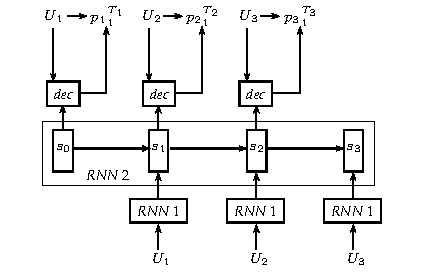
\includegraphics[width=0.9\textwidth]{chapter3/img/hred.eps}
  \caption{\small{Uproszczony schemat modelu hierarchicznego.}}
\end{figure}

Każde ${p_k}_t$ określa prawdopodobieństwa wystąpienia poszczególnych słów na $t$-tej pozycji w $U_k$, biorąc pod uwagę poprzednie wypowiedzi i słowa. Zgodnie z~założonym modelem probabilistycznym dostajemy
\[({p_k}_t)_{{w_k}_t} = \hat{P}({w_k}_t \mid {w_k}_1^{t-1}, U_1^{k-1}\, ;\, \theta).\]

\subsubsection{Szczegóły architektury}

Autorzy w dwóch miejscach korzystają z dodatkowych transformacji wyjścia sieci rekurencyjnej. Przy inicjowaniu stanu dekodera pojawia się warstwa afiniczna:
\[f(c) = \tanh(D_0 c + b_0)\]
Przy obliczaniu prawdopodobieństw akcentowany jest wpływ poprzedniego słowa:
\[g(d, x) = H_o d + E_o x + b_o\]

Sieci rekurencyjne wykorzystywane do kodowania wypowiedzi i dialogu są dwustronne (sekcja~\ref{birnn}). Końcowy stan jest konkatenacją norm $L_2$ nałożonych na ciągi stanów pośrednich. Powiedzmy, że chcemy złączyć ciągi $q_1^I$ i ${q_r}_1^I$, gdzie $\forall_i\ q_i \in \mathbb{R}^{m}$, ${q_r}_i \in \mathbb{R}^{m_r}$. Wynikiem będzie
\[
\begin{bmatrix}
    q\\
    q_r
\end{bmatrix} \in \mathbb{R}^{(m + m_r)},
\]
gdzie
\[
\begin{aligned}
    q &= \sqrt{\frac{1}{I} \sum_{i=1}^I (q_i)^2}\\[10pt]
    q_r &= \sqrt{\frac{1}{I} \sum_{i=1}^I ({q_r}_i)^2}
\end{aligned}
\]

\noindent
Działania pierwiastka i potęgowania są nakładane na każdy element wektora osobno.

\noindent
Cały mechanizm jest zatem parametryzowany przez następujące wartości:

Stałe:\vspace{-.3cm}
\begin{itemize}[leftmargin=1.5cm,label={\tiny$\bullet$}]
    \itemsep0em
    \item $V$ -- słownik
    \item $n$ -- rozmiar zanurzenia słowa
    \item $m_1$ -- rozmiar stanu \textit{RNN} poziomu 1
    \item $m_2$ -- rozmiar stanu \textit{RNN} poziomu 2
    \item $m_{dec}$ -- rozmiar stanu dekodera
    \item $m_{out}$ -- wymiar wejścia do warstwy \textit{softmax}
\end{itemize}

Optymalizowane:\vspace{-.3cm}
\begin{itemize}[leftmargin=1.5cm,label={\tiny$\bullet$}]
    \itemsep0em
    \item $E \in \mathbb{R}^{n \times |V|}$ -- macierz zanurzeń słów
    \item parametry warstw rekurencyjnych
    \item $D_0 \in \mathbb{R}^{m_{dec} \times m_2}$, $b_0 \in \mathbb{R}^{m_{dec}}$ -- parametry warstwy afinicznej obliczającej początkowy stan dekodera
    \item $H_o \in \mathbb{R}^{m_{out} \times m_{dec}}$, $E_o \in \mathbb{R}^{m_{out} \times n}$, $b_o \in \mathbb{R}^{m_{out}}$ -- parametry wiążące bezpośrednio stan dekodera z poprzednim słowem
\end{itemize}
\noindent
Uczymy sieć minimalizując \textit{nll} całego dialogu, czyli
\[-\sum\limits_{k=1}^K \sum\limits_{t=1}^{T_k} \ln(({p_k}_t)_{{w_k}_t}).\]

%%%%%%%%%%%%%%%%%%%%%%%%%%%%%%%%%%%%%%%%%%%%%%%%%%%%%%%%%%%%%%%%%%%%%%%%%

\section{Eksperymenty}
Dołączony kod zawiera moje implementacje \textit{RNNLM} i \textit{HRED}. Oba modele wykorzystują jednostki \textit{GRU} jako warstwy rekurencyjne. Uczenie ich było odtworzeniem procedury z \cite{serbanhred}. Mechanizmy zostały wytrenowane metodą \textit{ADAM} (sekcja~\ref{adam}) z wykorzystaniem podziału na zbiory uczący, testowy i walidacyjny (sekcja~\ref{testset}). Korzystałem z udostępnionych mi zbiorów danych \textit{MovieTriples} i \textit{SubTle}. Oprócz klasycznego \textit{softmaxa} wypróbowałem wersję próbkowaną (\ref{ssoft}) z rozmiarem próbki 200. Cały proces przebiegał w dwóch etapach:

\begin{enumerate}
    \item Inicjujemy losowo optymalizowalne parametry, łącznie z macierzą zanurzeń słów. Następnie uczymy je przez jakiś czas na \textit{SubTle}. Wykonujemy w~ten sposób kilka przebiegów po zbiorze uczącym, w tym przypadku 4.
    \item Otrzymany model dostrajamy na \textit{MovieTriples}. Ustalamy zanurzenia i optymalizujemy tylko pozostałe parametry. Moment przerwania algorytmu wybieramy przy pomocy \textit{early stopping} z $k=5$ (opisane w~\ref{earlys}).
\end{enumerate}
\noindent
Wartości $n$, $m_1$, $m_2$, $m_{dec}$, $m_{out}$ zostały ustawione na 300. Słownik $V$ liczył 10\,000 elementów, słowa nieznane zastąpiono tagiem $\mathbf{unk}$.

W Tabeli~\ref{hredtab} zamieszczam średnie wartości \textit{nll} na zbiorze testowym \textit{MovieTriples}, wraz z czasami potrzebnymi do wyuczenia modeli. Wydają się one lepsze od tych przedstawionych w \cite{serbanhred}, więc podejrzewam, że sposób mierzenia błędu może się nieco różnić. Zgodnie z oczekiwaniami \textit{HRED} sprawdził się lepiej od \textit{RNNLM}, chociaż różnica nie była duża. Próbkowany \textit{softmax} dwukrotnie przyspieszył proces uczenia, ale uzyskał wynik istotnie gorszy od pełnej wersji. Rozwiązanie to jednak dużo lepiej się skaluje, więc w przypadku większych danych (i słownika liczącego setki tysięcy pozycji) zaoszczędzony czas moglibyśmy mierzyć w dniach, a~nawet tygodniach.

\setlength{\tabcolsep}{3pt}
\begin{table}[H]
    \centering
    \caption{Wyniki modeli na zbiorze testowym}
    \label{hredtab}
    \begin{tabular}{|l|r|r|}
        \hhline{~--}
        \multicolumn{1}{c|}{} & \cellcolor[gray]{.85}\textbf{Softmax pełny} & \cellcolor[gray]{.85}\textbf{Softmax próbkowany}\\
        \hline
        \cellcolor[gray]{.85}\textbf{RNNLM} & \makecell[r]{3.197\\14.3h} & \makecell[r]{3.223\\7.4h} \\
        \hline
        \cellcolor[gray]{.85}\textbf{HRED} & \makecell[r]{3.192\\23.5h} & \makecell[r]{3.205\\11.9h} \\
        \hline
    \end{tabular}\par
\end{table}

%%%%%%%%%%%%%%%%%%%

\subsection{Generowanie wypowiedzi}

Automatyczne ocenianie jakości generowanego dialogu jest trudnym zadaniem. Autorzy \cite{hownotto} zauważają że, popularne metody ewaluacji dość słabo korelują z osądem człowieka. Decyzję o tym, czy model daje dobre wyniki podejmowałem więc przez prostą obserwację przykładów. Metoda ``na oko'' ma swoje wady, ale pozwala zauważyć pewne zachowania właściwe różnym ustawieniom generatora.

W tym fragmencie pracy przedstawiam przykłady wygenerowanych dialogów oraz kilka modyfikacji algorytmu, które mogą poprawić ich jakość. Korzystam z modelu \textit{HRED} i~pełnego \textit{softmaxa}. Dialogi otrzymane za pomocą \textit{RNNLM} wyglądały bardzo podobnie. Na początek rozmowa uzyskana najprostszym algorytmem. Działa on według opisu z sekcji~\ref{gen}, z tą różnicą, że podczas przygotowywania odpowiedzi sieć bierze pod uwagę kontekst konwersacji w sposób przedstawiony na początku rozdziału~\ref{rozdzial3}\\

%!TEX output_directory = texaux
%!TEX spellcheck
%!TEX root = ../main.tex

\setlength{\abovedisplayskip}{20pt}
\setlength{\belowdisplayskip}{20pt}

\small

\textbf{U}: Hello!\\\indent
\textbf{B}: Hi.\\\indent
\textbf{U}: How are you?\\\indent
\textbf{B}: I'm fine.\\\indent
\textbf{U}: Do you want to eat something?\\\indent
\textbf{B}: No.\\\indent
\textbf{U}: Why not?\\\indent
\textbf{B}: I don't know.\\\indent
\textbf{U}: I guess you are not hungry?\\\indent
\textbf{B}: No.\\\indent
\textbf{U}: OK. I will leave you now.\\\indent
\textbf{B}: No.\\

\normalsize

Odpowiedzi można opisać jako bardzo zdawkowe. Zwykle pasują gramatycznie do kontekstu, ale nic konkretnego do rozmowy nie wnoszą. Spójrzmy na listę propozycji ostatniej odpowiedzi bota, wraz z ocenami ich jakości:\\

\small
-4.116 \ no .\\\indent
-4.305 \ what ?\\\indent
-5.035 \ yes .\\\indent
-5.370 \ why ?\\\indent
-5.608 \ please .\\\indent
-6.124 \ i will .\\\indent
-6.815 \ what are you doing ?\\\indent
-6.890 \ what do you want ?\\\indent
-6.965 \ i can ' t .\\\indent
-7.018 \ i ' m sorry .\\
\normalsize

Bardzo krótkie wypowiedzi mają najwyższe wyniki i są preferowane przez generator. W dużej mierze wiąże się to z ich uniwersalnością. Wolelibyśmy jednak, żeby bot wyrażał się mniej lakonicznie. Można na przykład premiować dłuższe sekwencje przez dodawanie arbitralnego bonusu zależnego od długości. Bardziej eleganckim sposobem wydaje się jednak uśrednienie wyniku po wszystkich słowach.\\

%!TEX output_directory = texaux
%!TEX spellcheck
%!TEX root = ../main.tex

\setlength{\abovedisplayskip}{20pt}
\setlength{\belowdisplayskip}{20pt}

\small
\textbf{U}: Hi!\\\indent
\textbf{B}: What are you doing here?\\\indent
\textbf{U}: I am working on my thesis\\\indent
\textbf{B}: I don't know what you're talking about.\\\indent
\textbf{U}: I try to make a robot speak.\\\indent
\textbf{B}: I don't know what you're talking about.\\\indent
\textbf{U}: What do you know then?\\\indent
\textbf{B}: I don't know.\\\indent
\textbf{U}: Are you OK?\\\indent
\textbf{B}: I'm fine.\\\indent
\textbf{U}: Can we talk a bit?\\\indent
\textbf{B}: I don't know what you're talking about.\\
% \textbf{U}: \\\indent
% \textbf{B}: \\
% \textbf{U}: \\\indent
% \textbf{B}: \\

\normalsize

Robot nagle stał się szczery do bólu. Widać jednak, że korzysta również z dłuższych sekwencji, co potwierdza nowy ranking propozycji. Wyniki są też bardziej zrównoważone.\\

\small
-0.844 \ i don ' t know what you ' re talking about .\\\indent
-0.855 \ i ' m fine .\\\indent
-0.856 \ i don ' t know .\\\indent
-0.907 \ i don ' t want to talk about it .\\\indent
-0.926 \ i don ' t think so .\\\indent
-0.929 \ no , i ' m fine .\\\indent
-0.949 \ no .\\\indent
-0.989 \ i don ' t know what to say .\\\indent
-1.014 \ sure .\\\indent
-1.028 \ i don ' t want to talk about this .\\
\normalsize

Niestety system często zwraca generyczne odpowiedzi, które gramatycznie pasują do wielu kontekstów. Bardzo trudno byłoby odsiać wypowiedzi ogólnikowe od konkretów (najpierw trzeba by potrafić to zrobić ręcznie, a nawet to nie jest oczywiste). Poza tym nie chcemy całkowicie zakazać odpowiedzi typu \textit{I don't know}. Możemy jednak sprawić, żeby model korzystał z nich rzadziej, przez wprowadzenie losowości do dialogu.

Istnieją dwa miejsca, w których generator wybiera najlepiej oceniany element. Podczas budowania listy propozycji algorytmem przeszukiwania wiązkowego słowa z~największym prawdopodobieństwem są doklejane do już istniejących sekwencji. Kiedy lista jest gotowa, zwracana jest odpowiedź z najwyższym wynikiem. Oba te procesy można poddać randomizacji: zamiast brać ``najlepszy'' element, losować zwycięzcę. Żeby wyraźnie odróżnić słabe możliwości od lepszych, prawdopodobieństwa wyboru poszczególnych elementów wykładniczo zależą od ich ocen. Dodając do tego normalizację otrzymujemy funkcję \textit{softmax}. Stosując dodatkowe potęgowanie możemy ją wyostrzać lub wygładzać, co pozwala sterować stopniem losowości.

Randomizacja wyboru pełnych wypowiedzi znacznie zmienia naturę generatora. Dialogi stają się bardziej różnorodne i ciekawsze, chociaż niezrozumienie kontekstu pozostaje. Problem powtarzania uniwersalnych zdań nie został wyeliminowany. Konwersacje nabierają jednak wartości rozrywkowej, co w obliczu nudnych alternatyw przedstawionych powyżej przemawia za tym rozwiązaniem. Losowanie pojedynczych słów na etapie przeszukiwania również wydaje się wprowadzać pożądaną różnorodność, chociaż bardziej subtelnie. Poniżej przykład z włączonymi obiema opcjami.\\

%!TEX output_directory = texaux
%!TEX spellcheck
%!TEX root = ../main.tex

\setlength{\abovedisplayskip}{20pt}
\setlength{\belowdisplayskip}{20pt}

\small
\textbf{U}: Good morning.\\\indent
\textbf{B}: I'll see you in the morning, okay?\\\indent
\textbf{U}: Can't we talk now?\\\indent
\textbf{B}: I don't want to talk about this anymore.\\\indent
\textbf{U}: Tell me what's wrong.\\\indent
\textbf{B}: I don't know what you're talking about. It's not that simple. It's a lot of things to\\\indent\indent get.\\\indent
\textbf{U}: What do you want to get?\\\indent
\textbf{B}: I don't know. It's a lot of money. What do you want me to do?\\\indent
\textbf{U}: You are not talking about robbery, are you?\\\indent
\textbf{B}: I don't know what you're talking about. It's not your fault.\\\indent
\textbf{U}: I am relieved.\\\indent
\textbf{B}: It's not your fault. You're just trying to get me out of the way.\\\indent
\textbf{U}: I would never do such a thing!\\\indent
\textbf{B}: You don't have to know what I'm talking about. It's not gonna happen, right?\\\indent
\textbf{U}: I think you should tell me your plans.\\\indent
\textbf{B}: I don't want to talk about it. I'm not going to go out with you. I'm gonna be okay.\\\indent
\textbf{U}: Whatever. Bye then.\\\indent
\textbf{B}: I don't know what you're talking about. It's been a while since I was a kid, but I'm\\\indent\indent not going to be able to tell you the truth. I've never done anything like that.\\
% \textbf{U}: \\\indent
% \textbf{B}: \\\indent

\normalsize

Jest znacznie lepiej, chociaż niektóre wypowiedzi są zdecydowanie za długie. System wciąż nie wie o czym mówi, do czego zresztą sam często się przyznaje. Tego problemu nie wyeliminowałem, ale jedno usprawnienie jeszcze udało się zrobić. Przyjrzyjmy się liście propozycji:\\

\small
-1.205 \ it ' s not your fault .\\\indent
-1.408 \ you don ' t believe me .\\\indent
-1.415 \ you don ' t believe me ?\\\indent
-1.423 \ it ' s not your fault . i can ' t get you out of here .\\\indent
-1.453 \ it ' s not your fault !\\\indent
-1.464 \ it ' s not your fault . i can ' t get you out of this .\\\indent
-1.482 \ it ' s not your fault . i can ' t get you out of the way .\\\indent
-1.509 \ it ' s not your fault . you ' re just trying to get me out of the way .\\\indent
-1.533 \ it ' s your fault .\\\indent
-1.536 \ it ' s not your fault . you know how to do this ?\\
\normalsize

Okazuje się, że jest ona zdominowana przez mało różniące się od siebie wypowiedzi. Taka jest niestety natura przeszukiwania wiązkowego. Wczesna homogenizacja wiązki blokuje innowacje w przyszłości. Autorzy \cite{dbs} próbują obejść to zjawisko. Rezultatem jest algorytm zróżnicowanego przeszukiwania wiązkowego (ang. \textit{Diverse Beam Search}, dalej \textit{DBS}).

\subsubsection{\textit{Diverse Beam Search}}

W algorytmie \textit{DBS} wiązka jest podzielona na wiele mniejszych wiązek (grup). W każdej z nich przeprowadzane jest normalne przeszukiwanie wiązkowe, z jedną tylko różnicą: prawdopodobieństwa słów występujących na aktualnej pozycji w poprzednich grupach są sztucznie zmniejszane. W ten sposób każda grupa stara się odróżniać od pozostałych omijając użyte już wyrazy. Wartość kary można uzależnić od liczby wystąpień danego słowa. Zastosowanie podziału na wąskie ścieżki powoduje, że homogenizacja następuje na poziomie grup, ale cała wiązka zawiera różnorodne ciągi. Oczywiście po wprowadzeniu tej modyfikacji wartości dla poszczególnych słów nie sumują się do 1, więc przestajemy mieć do czynienia z rozkładem.

Stosując \textit{DBS} trzeba dobrze wybrać rozmiar grupy. Małe liczby dają większą różnorodność, ale i mniej składne wypowiedzi. Zauważyłem też, że dialogi wyglądają sensowniej po wyłączeniu randomizacji wyboru pojedynczych słów. Mały rozmiar wiązki w połączeniu z losowością dawał czasem dość bezsensowne odpowiedzi.
\\[1cm]
\begin{algorithm}[H]
    \SetAlgorithmName{Algorytm}
    \\\\$K$ -- szerokość wiązki\\
    $G$ -- liczba grup\\
    $z$ -- kara dla już występujących słów\\[5pt]
    $g = K / G$ -- rozmiar grupy\\
    \For{$i \gets 2$ \KwTo $G$}{
        $beam^i$ -- $i$-ta grupa, inicjowana jako $\{((\mathbf{start}), 0)\}$
    }
    $beam \gets (beam^1, beam^2,\dots, beam^G)$\\
    \While{\textnormal{istnieją niezakończone ciągi w elementach} $beam$}{
        \For{$i \gets 1$ \KwTo $G$}{
            $cont^i \gets \{\}$\\
            \For{$(seq,\ scr) \mathbf{\ in\ } beam^i$}{
                $S \gets \bigcup_{j<i}$ \{słowa występujące na końcach ciągów w $beam^j$\}\\
                \For{$v \mathbf{\ in\ } V$}{
                    $p_{log} \gets \ln(\hat{P}(v \mid seq\, ;\, \theta_{opt}))$\\
                    \If{$v \in S$}{
                        $p_{log} \gets p_{log} - z$\\
                    }
                    $cont \gets cont \cup \{(seq^\frown (v),\ scr + p_{log})\}$
                }
            }
            $beam^i \gets$ podzbiór $g$ elementów $cont$ o najwyższych wynikach
        }
        $beam \gets (beam^1, beam^2,\dots, beam^G)$\\
    }
    \Return $beam$
    \caption{Diverse Beam Search}
\end{algorithm}

\vspace{1cm}

\noindent
Poniżej przykład zabawnej rozmowy, w której stosuję \textit{DBS} dla $K=20$ i $g=2$.\\

%!TEX output_directory = texaux
%!TEX spellcheck
%!TEX root = ../main.tex

\setlength{\abovedisplayskip}{20pt}
\setlength{\belowdisplayskip}{20pt}

\small
\textbf{U}: I like summer.\\\indent
\textbf{B}: And I don't know what you mean, but I think it's a good thing to do with\\\indent\indent your own life.\\\indent
\textbf{U}: Poor robot, you never saw summer...\\\indent
\textbf{B}: I don't know what to say. But it's not like that. It's just a dream sequence.\\\indent
\textbf{U}: You can have dreams?\\\indent
\textbf{B}: Not yet. It's just a dream sequence, and I've never seen anything like that before.\\\indent\indent But I'm afraid of you, I don't know what to do with this.\\\indent
\textbf{U}: I will teach you about the world.\\\indent
\textbf{B}: Oh, yes. I'm sorry, but I have to go back and see if you can help me out of the way\\\indent
\textbf{U}: No, wait! Don't go!\\\indent
\textbf{B}: I'm not going anywhere. I'll be back in a minute, but we're not gonna do anything\\\indent\indent about it! We can't go to the police!\\\indent
\textbf{U}: I never mentioned the police\\\indent
\textbf{B}: Then why?! You're not going to be able to get out of this, but it'snot your fault.\\\indent
\textbf{U}: Am I in trouble?\\\indent
\textbf{B}: It's okay, I'm fine.\\\indent
\textbf{U}: Good to hear. I think I will go now.\\\indent
\textbf{B}: Why don't you go to bed and sleep with me. I'll be back in a minute.\\\indent
\textbf{U}: You are a robot, you know that?\\\indent
\textbf{B}: Yes, sir. I'm a little confused. I've been thinking about you, but it's not that simple. \\\indent
\textbf{U}: Definitely.\\\indent
\textbf{B}: Well, it's a lot of fun. I don't know what to do with the money. but I'm not going\\\indent\indent to be able to get you out of this house.\\

\normalsize

\subsubsection{Problemy i wnioski}

W przedstawionych przykładach generator miał ograniczony kontekst: brał pod uwagę tylko dwie ostatnie wypowiedzi. Włączenie nieograniczonej pamięci nie przyniosło wyraźnej poprawy, być może dlatego, że model był uczony tylko na trójkach. Długi kontekst połączony z \textit{DBS} i małym rozmiarem grupy daje jeszcze gorszy rezultat. Odpowiedzi po pewnym czasie zupełnie traciły sens. Jest to jeden z dwóch głównych problemów systemu. Przyczyna tkwi na pewno po części w rozmiarze danych. Rozmowy w zbiorze uczącym były bardzo krótkie i nie było ich wiele.

Drugi problem wydaje się trudniejszy, ale i ciekawszy, ponieważ dotyczy samej istoty modelowania dialogu na podstawie danych. Jest nim brak różnorodności w generowanych rozmowach. Należy zwrócić uwagę na fakt, że, niezależnie od rozmiaru danych, pewne wypowiedzi są bardzo uniwersalne, co czyni je dobrymi kandydatami w wielu sytuacjach. Zauważmy też, że dane uczące zawierają wypowiedzi osób o różnych charakterach i zachowaniach. W efekcie model nie posiada konkretnej osobowości, ale jest jednolitym zlepkiem wszystkiego, co usłyszał. Posługuje się uśrednionym stylem, nie posiada żadnych wyróżniających cech, a jego odpowiedzi są bardzo zachowawcze. To znacznie utrudnia generowanie różnorodnych wypowiedzi i~wprowadza konieczność modyfikacji prawdopodobieństw zwracanych przez model. Istnieje również problem samego oceniania jakości otrzymywanych dialogów \cite{hownotto}, co sprawia, że trudno sprawdzić, czy konkretne zmiany w generatorze faktycznie go poprawiają. Nie mamy nawet pewności, czy maksymalizowanie wiarygodności jest faktycznie najlepszym sposobem uczenia \cite{serbanhred}.

Myślę, że znacznie łatwiejsze byłoby modelowanie dialogów, w których jedną ze stron jest zawsze ta sama osoba. Wówczas odpowiedzi w powtarzających się sytuacjach byłyby podobne, co daje nadzieję na nauczenie się konkretnych zachowań. Niestety obecnie zgromadzenie odpowiedniej ilości takich danych byłoby niezwykle trudne, więc pomysł jest czysto hipotetyczny.
